\documentclass{article}
\usepackage{fancyvrb}
\usepackage{xcolor}
\usepackage{pygments}

\usepackage{polytexnic}
\begin{document}

\title{The Tau Manifesto}
\author{Michael Hartl}
\date{June 28 (``Tau Day''), 2010}
\maketitle

\section{The most important number} % (fold)
\label{sec:the_most_important_number}

Welcome to the \emph{Tau Manifesto}. This manifesto is dedicated to one of the most important numbers in mathematics---perhaps \emph{the} most important number: the \emph{circle constant} relating the circumference of a circle to its linear dimension. For millennia, circles have been considered the most perfect of shapes, and the circle constant captures the geometry of the circle in a single number. Surely, defining this number properly is a task that the great mathematicians of history should---nay, \emph{must}---have gotten right\ldots

Only they didn't.  As mathematician Bob Palais noted in the article ``$\pi$ Is Wrong!''\footnote{Palais, Robert. ``$\pi$ Is Wrong!'', \emph{The Mathematical Intelligencer}, Volume~23, Number~3, 2001, pp.~7--8. Available online \href{http://www.math.utah.edu/~palais/pi.html}{here}.}, $\pi$ \emph{is wrong}. The traditional definition for the circle constant sets $\pi$ (pi) equal to the ratio of the circle's circumference to its diameter:


\[
  \pi = \frac{C}{D} = 3.14159265\ldots
\]

\noindent Unfortunately, this definition is off by a factor of two. A circle is the set of points a fixed distance---the \emph{radius}---from a given point, so the most natural definition for the circle constant uses $r$ in place of $D = 2r$:

\[
  \mathrm{circle\ constant} = \frac{C}{r}
\]

Although his arguments are persuasive, even the plucky Professor Palais couldn't quite bring himself to take his idea completely seriously; instead of using a proper letter, he introduced a weird three-legged symbol for the circle constant (\hyperref[fig:palais-tau]{Figure~}\ref{fig:palais-tau}), which he called ``one turn''. As we'll see, the description is prescient, but the symbol, lamentably, is a non-starter.


\begin{figure}
\begin{center}

\includegraphics{images/figures/palais-tau.png}
\end{center}
\caption{The strange symbol used for the circle constant in ``$\pi$ Is Wrong!''.\label{fig:palais-tau}}
\end{figure}

The \emph{Tau Manifesto} is dedicated to the following proposition: the proper response to ``$\pi$ is wrong'' is ``No, \emph{really}.'' And the true circle constant deserves a proper name. The \emph{Tau Manifesto} proposes that this name---as I hope you will not be surprised to learn---should be the Greek letter $\tau$ (tau):

\[
  \tau = \frac{C}{r} = 6.2831853071796586\ldots
\]


 \subsection{Pro-pi propaganda} % (fold)

Before proceeding with the demonstration that $\tau$ is the natural choice for the circle constant, let us first acknowledge what we are up against---for there is a powerful conspiracy, centuries in the making, determined to propagate pro-$\pi$ propaganda. Entire \href{http://www.amazon.com/exec/obidos/ISBN=0802713327/parallaxproductiA/}{books} \href{http://www.amazon.com/Pi-Sky-Counting-Thinking-Being/dp/0198539568}{are} \href{http://www.amazon.com/exec/obidos/ISBN=0312381859/parallaxproductiA/}{written} extolling the virtues of $\pi$. I mean, \href{http://www.amazon.com/exec/obidos/ISBN=0387989463/parallaxproductiA/}{\emph{books}}\emph{!} And $\pi$ perfidy has captured even the highest levels of geekdom; for example, for the 2010 ``$\pi$ Day'' celebration (taking place on March~14), Google \emph{changed its logo} to honor $\pi$  (\hyperref[fig:google-pi-day]{Figure~}\ref{fig:google-pi-day}).  Meanwhile, some people memorize dozens, hundreds, even \emph{thousands} of digits of this mystical number. What kind of sad sack memorizes dozens of digits of $\pi$ (\hyperref[fig:michael_hartl]{Figure~}\ref{fig:michael_hartl})?

\begin{figure}
\begin{center}
\image{images/figures/google-pi-day.gif}
\end{center}
\caption{The Google logo on March 14, 2010.\label{fig:google-pi-day}}
\end{figure}

\begin{figure}
\begin{center}
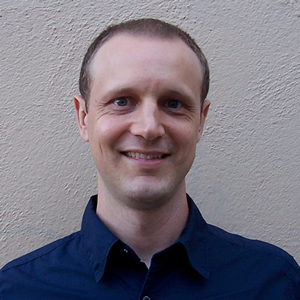
\includegraphics{images/figures/michael_hartl.jpg}
\end{center}
\caption{This poor bastard once memorized $\pi$ to 50 decimal places.\label{fig:michael_hartl}}
\end{figure}

Truly, we face a might opponent. Luckily, we have a powerful ally: the truth is on our side.

% section the_most_important_number (end)

\section{The nature of angle} % (fold)

Look through 

and you see...

But the best demonstration ...

Students of trigonometry learn special angles (\hyperref[fig:degree-angles]{Figure~}\ref{fig:degree-angles}).

\begin{figure}
\begin{center}
\image{images/figures/degree-angles.png}
\end{center}
\caption{Some important angles, in degrees.\label{fig:degree-angles}}
\end{figure}

Degrees break circles arbitrarily into 360 equal parts. More natural is to note that, since 

The arclengths differ, but the \emph{ratio} of the arclength to the radius is the same for each. This suggests the following definition of \emph{radian angle measure}:

\[ \theta = \frac{s}{r} \]

If you recall high-school trig, you probably have the special angles shown in \hyperref[fig:pi-angles]{Figure~}\ref{fig:pi-angles} floating around in your brain. I call this system of measure $\pi$-radians to emphasize that they are written in terms of $\pi$.

\begin{figure}
\begin{center}
\image{images/figures/pi-angles.png}
\end{center}
\caption{Some important angles, in $\pi$-radians.\label{fig:pi-angles}}
\end{figure}

Just how stupid is $\pi$? A moment's reflection shows that the so-called ``special'' angles are simply  \emph{rational fractions} of a full circle, as shown in \hyperref[fig:angle-fractions]{Figure~}\ref{fig:angle-fractions}.

\begin{figure}
\begin{center}
\image{images/figures/angle-fractions.png}
\end{center}
\caption{The ``important'' angles are rational fractions of a full circle.\label{fig:angle-fractions}}
\end{figure}

\noindent We can now revisit the definition of radian angle measure, rewriting it in terms of the fraction \emph{f} as follows:\footnote{The $\equiv$ symbol means ``is defined as''.}

\[ \theta = f\,\frac{C}{r} \equiv f\tau \]

\noindent Note how naturally $\tau$ falls out of this analysis. The resulting diagram of angles---shown in \hyperref[fig:tau-angles]{Figure~}\ref{fig:tau-angles}---is a powerful argument in favor of $\tau$.
Indeed, upon comparing \hyperref[fig:tau-angles]{Figure~}\ref{fig:tau-angles} and \hyperref[fig:angle-fractions]{Figure~}\ref{fig:angle-fractions}, I consider it decisive.

\begin{figure}
\begin{center}
\image{images/figures/tau-angles.png}
\end{center}
\caption{Some important angles, in radians.\label{fig:tau-angles}}
\end{figure}

  \subsection{The circle functions} % (fold)
  \label{sec:the_circle_functions}

\begin{figure}
\begin{center}
\image{images/figures/sine-with-tau.png}
\end{center}
\caption{Important points for $\sin\theta$ in terms of the period $T$.\label{fig:sine-with-tau}}
\end{figure}

Lorem ipsum dolor sit amet, consectetur adipisicing elit, sed do eiusmod tempor incididunt ut labore et dolore magna aliqua. Ut enim ad minim veniam, quis nostrud exercitation ullamco laboris nisi ut aliquip ex ea commodo consequat. Duis aute irure dolor in reprehenderit in voluptate velit esse cillum dolore eu fugiat nulla pariatur. Excepteur sint occaecat cupidatat non proident, sunt in culpa qui officia deserunt mollit anim id est laborum.
  
  % subsection the_circle_functions (end)

% section radian_angle_measure (end)

Can write

\[ e^{i\theta} = \cos\theta + i\sin\theta \]

Evaluating at $\theta = \tau$ yields \emph{Euler's formula}:

\[ e^{i\tau} = 1 \]

(By the way, you may have seen Euler's formula written in terms of $\pi$ as 


\[ e^{i\pi} = -1 \]

\noindent But that minus sign is so ugly that the formula almost always rearranged immediately,\footnote{Where does that minus sign come from? It's almost as if it's trying to tell us something\ldots} yielding

\[ e^{i\pi} + 1 = 0 \]

\noindent At this point, the expositor usually makes some grandiose statement, noting that Euler's formula relates $0$, $1$, $e$, $i$, and $\pi$---sometimes called the ``five most important numbers of mathematics.'' And at this point, you might complain that Euler's formula with $\tau$ relates only four of those five. Fine:


\[ e^{i\tau} + 0 = 1 \]

Satisfied?)


In words, the equation

\[
  e^{i\tau} = 1
\]

\noindent makes the following fundamental observation: 

\begin{center}
\emph{The exponential of the imaginary unit times the circle constant is unity.} 
\end{center}

Since complex exponentials correspond to rotations in the complex plane, this can also be stated as follows:

\begin{center}
\emph{The complex exponential of the circle constant is one turn.}
\end{center}

\noindent As in the case of radian angle measure, we see how natural the association is between $\tau$ and one turn of a circle.


  \subsection{Why tau?} % (fold)
  \label{sec:why_tau}


\begin{enumerate}
  \item \textbf{No serious conflicts.} The symbol~$\tau$ is used for, e.g., \emph{strain} in mechanical engineering and \emph{proper time} in special and general relativity, but there is no universal conflicting usage.\footnote{Minor clashes are OK; after all, physicists manage to use $e$ both for the natural number and for the charge on an electron without causing apparent harm.} 
  
  \item \textbf{Physical resemblance.} $\tau$ is typographically similar to $\pi$, thereby evoking the proper image of a circle constant. Unfortunately, the number of ``legs'' isn't quite right: it would be poetic if we could write $\pi = 2\tau$, but it wasn't meant to be.\footnote{Of course, in that case $\pi$ would have the right definition, and we wouldn't have this manifesto.}
  
  \item \textbf{Etymology.} In the context of radian angle measure, $\tau$ represents one \emph{turn} of a circle. The root of the English word ``turn'' is the Greek word for ``lathe'', \emph{tornos}---or, as the Greeks would put it: 
  
\[ \tau \acute{o}\rho\nu o\varsigma \]
  
\end{enumerate}

\noindent Looking at the first letter of that Greek lathe, I'm going to go out on a limb here and say: \href{http://en.wikipedia.org/wiki/Q.E.D.}{\emph{quod erat demonstrandum}}.
  
  % subsection why_tau (end)


\section{Circular area} % (fold)
\label{sec:circular_area}

\[ A = \pi r^2 \]


Seems like the exception, but is really the coup de gr\^{a}ce.

\[ v \propto t \]

\[ v = g t \]

\[ y = \int_0^t gt\,dt = \textstyle{\frac{1}{2}} gt^2 \]


\[ F \propto x \]

\[ F = k x \]

\[ U = \int_0^x kx\,dx = \textstyle{\frac{1}{2}} kx^2 \]

\[ F \propto a \]

\[ F = m a \]

\[ K = \int ma\,dx = \int m\,\frac{dv}{dt}\,dx = \int m\, \frac{dx}{dt}\,dv = \int_0^v mv\,dv = \textstyle{\frac{1}{2}} mv^2 \]


\begin{figure}
\begin{center}
\image{images/figures/circular-area.png}
\end{center}
\caption{Calculating the area of a circle.\label{fig:circular-area}}
\end{figure}

\[ dA = C\,dr \]

\noindent But for a circle the circumference is proportional to the radius:

\[ C \propto r \]

\noindent The constant of proportionality is $\tau$:

\[ C = \tau r \]

\noindent The area of the full circle can then be calculated by integrating the differential element of area:

\[ A = \int dA = \int_0^r C\,dr = \int_0^r \tau r\,dr = \textstyle{\frac{1}{2}} \tau r^2 \]




% section circular_area (end)

\section{Puns}

We come now to the final objection: ``What about puns?'', I hear you cry. I know, I know, ``$\pi$ in the sky'' is so very clever. And yet, $\tau$ itself is pregnant with possibilities. After all, once you have accepted $\tau$ism, you will become a $\tau$ist like me. It is not $\tau$ that is a piece of $\pi$, but $\pi$ that is a piece of $\tau$---half~$\tau$, to be exact. This is the true nature of the~$\tau$.

\section{Conclusion}

We

About the author

Michael Hartl is an educator and entrepreneur. He is the creator of the  \href{http://www.railstutorial.org/}{Ruby on Rails Tutorial} and previously taught theoretical and computational physics at the \href{http://www.caltech.edu/}{California Institute of Technology} (Caltech), where he received the Lifetime Achievement Award for Excellence in Teaching in 2000. Michael knows 51 digits of $\pi$---i.e., fifty decimal places---approximately 48 more than Matt Groening. He is currently working on memorizing 53 digits of $\tau$.\footnote{It doesn't round off right if you truncate after 52 digits. But you probably figured that out already.}
\end{document}

